% Copyright (c) 2008-2009 solvethis
% Copyright (c) 2010-2016 Casper Ti. Vector
% Public domain.
%
% 使用前请先仔细阅读 pkuthss 和 biblatex-caspervector 的文档,
% 特别是其中的 FAQ 部分和用红色强调的部分。
% 两者可在终端/命令提示符中用
%   texdoc pkuthss
%   texdoc biblatex-caspervector
% 调出。

\documentclass[openany,UTF8]{pkuthss}
\usepackage{booktabs}
\usepackage[backend = biber, style = caspervector, utf8, sorting = none]{biblatex}
\AtBeginBibliography{\renewcommand*{\makelabel}[1]{#1\hss}}
\setlength{\bibitemsep}{3bp}
\setcounter{tocdepth}{1}
%\renewcommand*{\bibnumfmt}[1]{\makebox[3em][l]{[#1]}}
%\renewcommand{\bibnumfmt}[1]{\makebox[3em][l]{[#1]}}
\renewcommand*{\bibfont}{\zihao{5}\linespread{1.27}\selectfont}
\usepackage{url}
\usepackage{hyperref}
\hypersetup{
	colorlinks=true,
	linkcolor=black,
	filecolor=gray,      
	urlcolor=black,
	citecolor=black,
}
%\setcounter{tocdepth}{2}

\pkuthssinfo{
	cthesisname = {本科生毕业论文}, ethesisname = {Undergraduate Thesis},
	ctitle = {全自动加样系统的设计与开发}, 
    etitle = {},
	cauthor = {宋方腾},
	eauthor = {},
	studentid = {1502024142},
	date = {2019 年 5 月},
	school = {机械工程学院},
	cmajor = {机械设计制造及其自动化}, emajor = {},
	direction = {},
	cmentor = {成云平\quad 副教授}, ementor = {},
	ckeywords = {first second}, ekeywords = {First, Second}
}
\addbibresource{thesis.bib}

% 普通用户可删除此段,并相应地删除 chap/*.tex 中的
% “\pkuthssffaq % 中文测试文字。”一行。
\usepackage{color}
\def\pkuthssffaq{%
	\emph{\textcolor{red}{pkuthss 文档模版最常见问题:}}

	\texttt{\string\cite}、\texttt{\string\parencite} %
	和 \texttt{\string\supercite} 三个命令分别产生%
	未格式化的、带方括号的和上标且带方括号的引用标记:%
	\cite{test-en},\parencite{test-zh}、\supercite{test-en, test-zh}。

	若要避免章末空白页,请在调用 pkuthss 文档类时加入 \texttt{openany} 选项。

	如果编译时不出参考文献,
	请参考 \texttt{texdoc pkuthss}“问题及其解决”一章
	“其它可能存在的问题”一节中关于 biber 的说明。
}

\begin{document}
	\frontmatter
	\pagestyle{empty}
	\maketitle
	%\cleardoublepage
	\include{chap/copyright}

	% 此后到下一 \pagestyle 命令之前正常排版页眉和页脚。
	%\cleardoublepage
	\pagestyle{plain}
	% 重置页码计数器,用大写罗马数字排版此部分页码。
	\setcounter{page}{0}
	\pagenumbering{Roman}
	% 中英文摘要。
	\include{chap/abstract}
	% 自动生成目录。
	\tableofcontents
	\setcounter{tocdepth}{1}

	% 以下为正文部分,默认要进行章节编号。
	\mainmatter
	% 序言。
	% Copyright (c) 2014,2016 Casper Ti. Vector
% Public domain.

\chapter{序言}
\section{研究背景}
当今,人们愈加重视对疾病的预防和监测,而体外诊断是近些年来新兴并受到欢迎的一种有效监测手段和方法。它通过对某些人体样本(如体液、血液、组织液等)进行检测,判断其中是否存在疾病的生化标志物,从而及时的对疾病进行有效地掌控和治疗。体外诊断一种不可或缺的有机组成是血液的检测与分析,然而伴随着现代化进程的不断推进,人们不断增高的各种发病率使得进行血液样本分析的工作量剧增。与此同时,临床技术的发展也使得血液样本的分析从传统的手工操作到半自动化分析,进一步发展到现在的全自动检测。当今,最广泛使用的全自动血液测试和分析仪器是自动生化分析仪。它可用于临床生物化学的常规分析,以及对分泌激素,排泄物,脑脊液成分,有毒溶液和电解质的检测。这些测试为临床医学和科学研究实验提供了极大的便利。由于其强大的功能,全自动生化分析仪近年来已成为临床实验室分析中最常用的测试仪器。
\section{自动生化分析仪国内外研究现状}
自动生化分析仪是一种集多功能与一体的医学实验室仪器,它能够用于定量测量和分析人体血液,尿液和其他体液各种生物标志物和化学元素,如:微量元素和其他电解质,以及激素和微蛋白,并对肝功能,肾功能,心脏功能进行监测。人体液体生化指标具有重要的参考价值,它为临床医生在临床疾病诊断和治疗提供了原始数据。从全自动生化仪的 提出到现在大约半个世纪,生化分析仪得到了广泛的应用和迅速发展。目前在我国,生化分析仪的发展落后于先进国家。

自动生化分析仪在国外的研究起步于20世纪50年代,第一台自动生化分析仪诞生于瑞士。随着应用市场不断扩大,自动生化分析仪的研究迅速发展,其技术也日臻成熟,国外各龙头医疗器械企业都研制出自己的产品,比如瑞士的澳斯邦及帝肯、美国的强生、德国的西门子及罗氏、日本的奥林巴斯公司等等\supercite{bib2},这些国外科技势力发展迅速,这些国际龙头企业不断对自动生化分析仪硬件和软件系统进行更新,增加和完善了分析仪的许多功能,使检测仪器趋于完美。其产品具有加样速度快、位置精度高、抗干扰性强等优点。

我国对自动生化分析仪的研究开展比较晚,其起始于1972年引进美国泰克尼康公司流动式生化分析仪,在此基础上,我国研制出了第一台自动生化分析仪。上世纪八九十年代是我国自动生化分析仪发展的黄金时期,自动生化分析水平与国际先进水平之间的差距越来越小,但大多数的研发机器都处在样机阶段,不能进入应用市场。2003年,深圳奥迈Ominilab BS-300的面市才使得我国拥有了能商业化的全自动生化分析仪\supercite{bib1}。

在自动加样那个系统的相关研究中,文献\parencite{bib2}在完成机械机构、运动部件的设计和嵌入式控制的基础上,重点对加样系统关键的机械部件利用有限元软件进行了力学分析和功能仿真研究;文献\parencite{bib3}在搭建实验平台的基础上,重点研究了加样精度的控制算法和微量加样器的设计;文献\parencite{bib8}在完成自动加样系统的机械设计的基础上,通过对自动加样机的过载故障的研究,重点关注在步进电机细分驱动和调速控制上,并通过对正常组件和故障组件测量来验证效果;文献\parencite{bib9}在完成加样机械臂结构和尺寸的设计之后,重点建立相关数学模型进行了机械臂的运动学和动力学分析。这些研究成果均对自动加样系统的某一部分进行了重点研究,完善了加样系统设计方式,相比于半自动加样系统在加样效率有了一定的提高。然而,这些文献没有考虑控制成本及操作友好性,加样的精度和效率还有待提高。此外,设计的加样系统对小型研究团体没有针对性,存在体积大、部件价格贵、控制成本高等问题。
\section{论文研究意义及内容}
作为21世纪新的科研领域,自动生化分析仪的开发和应用受到医学,海关防疫,生物工程和生命科学等科技部门的高度重视。同时,需要处理的检测样本量指数式增加增加,使得实验人员面临的劳动强度十分严峻。全自动加样系统作为自动生化分析仪的核心部分,已成为朝着高精度和高质量发展的重点研究目标。

一般地,待测样本的加样量过小过大都会引起测定误差,进而影响试液最后的测定精度。一方面,我国的自动生化分析仪在加样精度指标上与国际先进水平样品加样的精度有很大的差距,国外领先水平的仪器加样最小分辨率达到了0.001$ml$数量级,而我国加样精度仍停留在0.05$ml$数量级。另一方面,国产自动生化分析仪存在灵敏度低、样本消耗多、控制系统精度差等诸多问题。因此,进行自动生化分析仪的自动加样系统的研究和设计的需求显得十分突出。而加快对自动加样系统的研究也有利于提升我国检测仪器的模块化发展,提高检测仪器系统部件的互换性,缩小与国际先进水平的差距,同时为人们健康提供有力的监测保障。此外,全自动加样系统的好处不仅包括减少医检实验人员手工劳动和操作危险试液所涉及的风险,还可以提高数据完整性,降低加样误差,提高准确性,加快分析过程,减少试液的耗用量从而降低成本,避免样品污染和人为错误。

当代检测技术对加样的准确性、重复性稳定性等要求越来越高。因此开展对全自动生化分析仪加样控制系统的研究,有利于提高国内全自动生化分析仪的设计生产水平以及测试准确性,推动国内样品检测技术、改善民众医疗服务条件。针对目前这一现状,为保证在保证一定加样精度的同时,提高加样效率、降低控制成本。本文设计了一种应用于自动生化分析仪的全自动加样系统,该系统的设计主要设计机电一体化技术、自动控制技术、传感器技术等。本文的研究在利用比较法、文献法、分析法、测试法基础上将以理论研究、软件、硬件分析与设计相结合的方式进行。将理论分析研究具体应用到控制方案中。具体如下:

第一章 ,查阅探究相关文献,论述全自动生化分析仪国内外发展状况,分析自动加样系统工作原理及相关技术,这是整个自动化加样系统设计的基础。

第二章,根据功能需求,设计自动加样系统的动作流程并确定系统相关的部件组成。

第三章,主要对加样机械臂的机械系统的设计,确定机械传动系统的驱动方式、传动方式和电机选型等,进行机械臂结构的设计。

第四章,据加样系统对定位控制要求,制定自动加样系统总体控制方案以及机械运动部分控制方案,包括根据励磁方式对步进电机选型,步进电机细分控制的分析,步进电机驱动器的分析与选型等。

第五章,根据控制方案和相关系统功能部件,进行硬件设计与选型,如下位机控制器的选取,驱动器的选取,绘制相关电路图。


% vim:ts=4:sw=4

	% 各章节。
	\chapter{自动加样系统总体方案的确定}
全自动生化分析仪是一个涉及到多种技术的复杂系统,具有多个功能模块,它的功用要求其具有精度高、可靠性高的特点。研制具有完全自主知识产权的全自动生化分析仪是十分困难的,其中的加样系统会直接影响到系统最后的测定的结果。因此,自动加样系统一直以来都是全自动生化分析仪的关键技术之一,它是一个典型的机电一体化产品,本文的研究对象即为全自动生化仪中的自动加样系统。本部分作为后续章节基础,根据自动加样系统的功用来阐述其基本组成部件,工作原理,硬件组成及控制方法。

\section{自动加样系统的分析}

自动加样系统常用于检测仪器中,其工作原理是上位机通过人机交互接收加样指令,下位机控制器解析指令控制系统动作,加样机构从样本盘和试剂盘中吸取样本和反应试剂,通过加样机械臂移送至指定位置;加样动作周期中一个重要的步骤是对加样针进行清洗,以避免试液之间的相互污染。从上述功用可知,自动加样系统一般由进行取样、释放样液(以下简称释样)的加样机构,完成加样功能的机械臂,起到人机交互功能的上位机,控制加样动作的下位机控制器,为防止试剂相互污染的清洗部件,用来盛放待检样液的样品盘以及放置反应试剂的加样盘组成。自动加样系统涉及到的主要技术机械结构设计、机电一体化、自动化控制,传感器等技术。

\section{加样机构的选定}
根据样品加样方式及其原理的不同,加样机构主要有三种结构\supercite{bib3},分别如下:

(1)蠕动泵加样结构。蠕动泵运用了手指挤压充满液体的软管的原理,设计者用滚轮替换手指,并在滚轮向前滚动时向前移动液体。通过交替挤压和释放柔性软管实现流体的运送。就像用手指捏住软管时,管内积聚负压汲取流体,当手指移动时,管内积聚正压排送流体,其工作原理图如\ref{fig:2-1}。

\begin{figure}[htbp!]
  \centering
  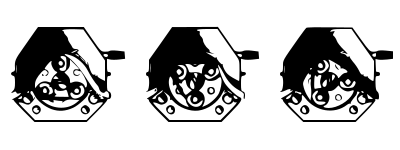
\includegraphics[height=3.5cm]{chap/figure/2-1.jpg}
  \caption{蠕动泵工作原理图}
  \label{fig:2-1}
\end{figure}

蠕动泵的特点明显:一方面,由于运送的材料只接触软管不接触外界环境,材料不易受外界环境的污染;其结构决定了蠕动泵的稳定精度好、运送真空度高;另外,不需要设置阀门机构,简化了结构同时又不会出现泄漏现象,也可用来泵送易阻塞、纤维质物料的流体\supercite{bib4},对运送材料形态要求低,运送材料种类广泛。只有软管是需要更换的部件,故更换、维护方便。另一方面,由于蠕动泵使用的软管硬度一定,故其承受压力会受到限制;并且,泵在滚轮交替运作时会产生一个脉冲流,从而导致发生回吸现象,有一定的加样误差。

(2)推入式加样结构。推入式加样结构是以手动加样为原理进行设计的。其动作过程为:从装有样液的试管内吸取一定的试液,移动至加样入口,将试液注入。这种结构设计非常简单,和医用注射器工作原理一致。使用时,高精度的步进电机带动丝杠配合具导向功能的注射滑块上的传动螺母为动力的传输方式,驱动注射器活塞做往返直线滑动,实现自动精密的定量加样。步进电机在数字脉冲信号响应下,作用于直线轴承实现直线往复运动\supercite{bib5}。此外,注射器的吸入和排出都在步进电机的控制下完成并且采用精密的结构件和合理的驱动方式,此方式可以实现高精度和高准确度,具有良好的稳定性与自动化控制,其结构原理图如\ref{fig:2-2}。

\begin{figure}[htbp!]
  \centering
  \includegraphics[height=4.8cm]{chap/figure/2-2.jpg}
  \caption{推入式自动加样结构工作原理图}
  \label{fig:2-2}
\end{figure}

(3)六通阀加样结构。该结构一般分为两类:一类是电机驱动的,另一类是用压缩气体驱动的。对于压缩气体驱动结构,利用气动阀内外的压力差,气动阀的一端连接气泵,取样时气动阀内为负压,释放样液时气动阀内为正压。由于采用气动阀,系统要保证良好的气密性,而一旦发生气体泄漏,会对实验分析造成很大的影响;对于电动结构来说:主要由控制部分和驱动部分组成,控制部分通过程序控制驱动部分的。从运动传动角度来看,电动通常属于直接式驱动,气动则属于间接式驱动。

六通阀加样结构一般用于气路加样机构,通过部分装液法或完全装液法进行加样。采用这两种方法对加样量均有要求。部分装液法加样法时,加样量一般是定量环体积的四分之三,且要保证每次相同的加样体积;采用完全装液法加样时,加样量最少为定量环体积的3至5倍从而高精密度、高重现性。此外,六通阀加样结构的清洗异常困难,通常用淡水稀释剂或流动液反复冲洗加样器,再用试纸擦净注射器针头。由此可知,六通阀自动加样结构对操作人员的加样操作要求高,难以保证加样精度和样液不受外界污染。该结构该结构的工作原理图如\ref{fig:2-3}。

\begin{figure}[htbp!]
  \centering
  \includegraphics[height=6.5cm]{chap/figure/2-3.jpg}
  \caption{六通阀自动加样结构工作原理图}
  \label{fig:2-3}
\end{figure}

综合比较以上三种加样结构,推入式自动加样结构具有复杂的设计要求,该结构采用丝杠传动且在加样的需求使得步进电机转动方向更换频繁,在此过程中即会出现回程误差,进而造成取样体积出现误差;注射器直接与待检试剂进行接触,不可避免会造成试剂的交叉污染从而造成重大实验损失;此外,该结构零部件更换不方便、难以进行调整以及维护。六通阀自动加样结构的加样阀易于遭受试剂样本中微粒的堵塞和磨损,生命周期短;每次使用前后都要对加样器进行反复的冲洗以避免交叉污染,操作复杂,工作效率低下。此外,六通阀自动加样结构对气密性具有较高的要求,容易受到操作环境变化的影响。而蠕动泵结构操作简单,去离子水和吸入的空气可以有效防止试剂的交叉污染,无加样阀不需要进行密的安全保障;关于运输压力的局限性,我们可以通过增加滚轮的数量降低流量从而降低对软管的压力,使用脉冲抑制器来减少甚至避免液体回吸,脉冲抑制器是一个简单的定位容器,它基于气体可压缩性强于液体可压缩性的工作原理,即脉冲流进入容器、液体上的气袋下陷吸收脉冲进而平缓的流出。当然它的最大缺点是软管易于磨损,但相比于其具有良好的性价比,这是可以接受的。综上所述,本设计的加样结构选用蠕动泵加样结构。

%蠕动泵在工作过程中滚轮会交替挤压软管,当滚轮离开软管%的瞬间会产生回吸现象。当进行加样时回吸现象会严重影响%加样精度,不适用于制造加样精度级高的全自动生化分析仪%。%



















   	% 各章节。
	\chapter{自动加样系统机械臂的设计}
自动加样系统能够实现的一个基本功用是在空间内平将待检样品和反应试剂用送到反应瓶内,实现任意位置的准确定位并且尽量减少加样时间同时保证运动的平稳。因此,自动加样系统的加样机械臂的设计十分重要和关键。本部分完成对其系统结构的设计。
\section{加样机械臂结构类型的选定}
机械臂结构类型多种多样,不同工作场景所使用的机械臂结构形式千差万别。工业上广泛使用的机械臂结构主要有以下几种:

1.铰接式结构:该设计由多个旋转接头和工作臂组成,从简单的双链接结构到多($5-8$个以上)相互作用的铰接系统。一般地,该结构在笛卡尔坐标系下能够实现三个转动自由度。一般情况下,铰接结构越多,工作范围越大,机械臂运动也就越精确。铰接式机械臂通常用于装配,压铸,气焊,及喷涂等工作场景。其机械结构简图如\ref{fig:3-1}。

\begin{figure}[htbp!]
	\centering
	\includegraphics[height=6.5cm]{chap/figure/3-1.jpg}
	\caption{铰接式结构简图}
	\label{fig:3-1}
\end{figure}

2.笛卡尔式结构:该结构在笛卡尔坐标系下一般有三个平动自由度,它能实现机械臂在空间内沿着$X,Y,Z$方向平动从而到达坐标系中任意位置。笛卡尔式机械臂通常用于装载(卸载)工件,印刷电子电路板,材料表面处理等工作场景。该结构提供的工作空间大(可用于其它用途)、控制系统简单。其机械结构简图如\ref{fig:3-2}。

\begin{figure}[htbp!]
	\centering
	\includegraphics[height=6.5cm]{chap/figure/3-2.jpg}
	\caption{笛卡尔式结构简图}
	\label{fig:3-2}
\end{figure}

3.圆柱式结构:该结构在笛卡尔坐标系统能实现沿着$X,Y$方向平动和绕$Z$方向转动,机器臂可以移动到由圆柱体描述的体积内的任意位置。该结构在垂直方向上节省了空间,具有良好的刚性能承受较大的有效载荷,但由于其结构限制不能实现$360$度转动。其机械结构简图如\ref{fig:3-3}。

\begin{figure}[htbp!]
	\centering
	\includegraphics[height=6.5cm]{chap/figure/3-3.jpg}
	\caption{圆柱式结构简图}
	\label{fig:3-3}
\end{figure}

4.极坐标式结构:该结构在笛卡尔坐标系下一般能够实现两个旋转自由度和一个平动自由度。相比于圆柱式结构,它在空间内能实现$360$度的转动,并且在水平方向上的工作距离更长。其机械结构简图如\ref{fig:3-4}。

\begin{figure}[htbp!]
	\centering
	\includegraphics[height=6.5cm]{chap/figure/3-4.jpg}
	\caption{极坐标式结构简图}
	\label{fig:3-4}
\end{figure}

根据加样系统的功用和动作流程,加样机械臂要能够到达三维空间中的任意位置;加样多孔板需要放置在工作台上,要求工作台空间足够大;加样液在移送过程中不能有滴漏,要求加样机械臂运动平稳;取样、释样过程不能发生样品(试剂)出错现象,要求加样机械臂运动精度高。考虑以上要素,综合对比上述四种机械臂结构本文选用笛卡尔式结构,该结构能够提供较大的工作空间,控制易于实现,运动平稳且精度高。
\section{驱动方式的选定}

加样机械臂的运动状态是由其驱动系统决定的,它一般由两个部分组成:驱动机构和传动机构。驱动机构其实质可以视为一种可以将其它能量如气动能量、电能等转化为加样机械臂的动能的装置,并通过传动机构使得机械臂动作。根据动力源的不同,可以将其分为电力源、液压源和气压源三种驱动类型。

电力驱动:该方式利用电动机产生的力矩和力驱动机械臂进行动作,其具有速度调节范围广、控制精度高、运动平稳性高的特点,具有良好的的控制性和环境适应性。常用的电机驱动器包括直流伺服电机、交流伺服电机、步进电机等。

液压驱动:该方式利用液体产生的压力驱动机械臂进行动作,其具有动力大,无级调速,能实现高速的精度控制等特点。但供油回油等附加元件使其系统体积大,成本高,维修困难,易泄漏对环境极度不友好、。该驱动方式多用于矿山机械,重型设备等。

气压驱动:该方式利用气体产生的压力驱动机械臂进行动作,其具有响应快清洁无害,易维护等特点。但其运动稳定性差,功率小,噪声大、难以实现较高精度的位置和速度控制,多用于小功率驱动、运动精度要求低的场合。

自动加样系统在加样过程中进行多次重复加样,位置重复性要求好;加样系统必须具有一定的效率,短时间内完成较多的加样任务,速度响应要求要好;加样过程中,为保证测试结果的准确度取样要准,运动平稳性和精度要求高。要求其运动平稳性好,位置精度高;其部件模块不大、负载小;并且,自动加样系统一般多用于医院、科研机构等对噪声要求严苛的地方。比较上述三种驱动方式,本文选用电力驱动。

进一步地,电力驱动所用的驱动器通常有直流伺服电机、交流伺服电机、步进电机。对于伺服电机,其主要特点是马达或执行机构上装有传感器,传感器将命令执行结果经由伺服放大器传回控制中心,控制中心在比较执行结果和指令值之后再对执行结果进行反馈纠正以不断减小运动执行误差。可以实现转速可以精确控制,速度控制范围广,除了可以进行稳定平顺等速运转之外,还可以根据需求随时变更速度。然而,一般伺服电机采取的控制方式是闭环控制,闭环系统中机械部件的惯性、传动误差、变形刚度等问题使得控制极其复杂和困难。而步进电机不用配备转角编码器等设备,且不受输入和输出因素的影响也不受冲击和振动等环境因素的影响;由脉冲信号控制执行机构运动的距离和速度,在不失步运行时步距累积误差为0,不需要位置检出和速度检出的回授元件,所以步进电机的输出可以由单一的脉冲的输入来决定,因此就能达成精确的位置和速度控制。另外,可以通过位置传感器(如限位开关)来辅助位置和速度的控制。步进电机对比伺服电机一个难以匹敌的优点是它使得本设计的系统体积小,结构紧凑。综合控制成本和控制效果来看,本文选择步进电机作为$X$、$Y$、$Z$方向平动的驱动器。

\section{传动方式选定}
加样机械臂传动方式对加样精度、稳定性和响应的快速性都产生重要影响。机械系统中传动机构多种多样,本文初步选定将步进电机的回转运动转换成直线运动的滚珠丝杠螺母传动和同步带。

滚珠丝杠螺母传动机构与一般的丝杠螺母副一致,但其在丝杠和螺母之间增加了滚珠。丝杠转动的同时滚珠也会在螺纹滚道里转动,滚珠又将运动传递给螺母,通过一系列的动作将转动量变换成平动量。滚珠丝杠螺母传动机构的传递的效率高,摩擦损失小,传动精度高但是其结构复杂、难以加工、制造困难;并且滚珠丝杠螺母机构需要润滑和密封机构以提高其工作效率和寿命。同步带传动是带传动和齿轮传动的有机结合体,兼备二者的优点。同步带的内周表面制有等距的距齿。工作时,利用带与带轮齿之间的啮合关系传递运动\supercite{bib7}。同步带的传动比准确且恒定,最吸引的一个优点是带的缓冲吸振特性使其传动平稳,结构紧凑,不需要密封和润滑维护方便,并且重量小,传动能量利用效率高,刚度影响因素少。

加样机械臂的传动比要求较高,传动过程不能发生干涉现象,尽量降低回程误差以提高传动精度,故选取同步带作为传动机构。此外,为保证加样过程中运动的平稳性和高精度,导性机构本设计采用滚动直线导轨。滚动直线导轨以适当滚珠放入滑块和导轨之间,这种设计使得滚动摩擦代替滑动摩擦从而减低了摩擦阻力,实现了高定位精度和重复精度。


\section{加样机械臂机械结构的设计}
本小结在以上分析的基础上进行笛卡尔式加样机械臂的结构绘制。经过分析可知,加样机械臂包括步进电机,同步带,滚动直线导轨

加样系统整体布局如图\ref{fig:3-5}
\begin{figure}[htbp!]
	\centering
	\includegraphics[height=8.5cm]{chap/figure/0.jpg}
	\caption{加样系统整体布局简图}
	\label{fig:3-5}
\end{figure}













































	% 各章节。
	\chapter{自动加样系统控制方案的确定}
\section{总体控制系统的确定}
自动加样的实现离不开各功能模块之间的配合,配合好坏的程度取决于控制系统的设计。该控制系统由上位机、下位机控制器,功率驱动器,步进电机,位置检测器,液位传感器组成。其中,上位机、下位机控制器进行加样动作指令的接收与解析且二者信息双向流通,功率驱动器和步进电机作为被控对象,位置传感器和液位传感器作为回授元件,进行控制反馈的输入量。自动加样控制系统的结构关系图如\ref{fig:4-1}。

\begin{figure}[htbp!]
	\centering
	\includegraphics[height=9.5cm]{chap/figure/4-1.jpg}
	\caption{自动加样控制系统的结构关系简图}
	\label{fig:4-1}
\end{figure}

从自动加样控制系统的结构关系简图可知,本控制方案采取了半闭环控制系统,采用位置传感器和液位传感器将被控元件的位置情况反馈给控制器以保证加样精度和位置准确度。

\section{步进电机类型的选择}
步进电机是一种由数字信号驱动、以一定周期进行的同步电机,简单来说步进电机就是将输入的脉冲信号转动成转角或直线距离输出。其种类多种多样,按工作原理主要可以分为永磁式($PM$型)、磁阻式($VR$型),永磁感应式($HB$型)三大种类\supercite{bib12}。步进电机运动精度依赖于其最小步距角(分辨率)。对于永磁式步进电机,其转子由永磁体制作,多为两相结构,输出转矩小,其分辨率一般为45$^ \circ $、90$^ \circ $及11.25$^ \circ $等几种。对于磁阻式步进电机,其转子由加工成齿状的软铁构成,无惯性转矩响应快,其负荷惯性较小,其分辨率一般为15$^ \circ $。对于永磁感应式步进电机,转子由轴向磁化的磁铁制成且具有复极式磁极,兼具永磁式和磁阻式两种电机的优点,精确度高、转矩大、步进角度小。本文选用永磁感应式(混合型)步进电机。

永磁感应式步进电机一般有两相、三向和五相三种类型,相数越多分辨率越小,运动精度越高,价格也越来越贵。考虑成本和控制效果,本设计拟采用两相混合式步进电机,其分辨率为1.8$^ \circ $,另外对分辨率进行细分以补偿运动精度。经调研,我们选取$Leetro$公司的产品$DM5641E$,该步进电机产品体积小巧,适合用于医疗仪器、电控平移台、各种分析仪器、医疗泵、横流泵、蠕动泵、注射泵、机械手\supercite{bib14}等各种中小型自动化设备和仪器。$DM5641E$步进电机的产品参数如下表\ref{tab:4-1},实物图如\ref{fig:4-8},电机接线图如\ref{fig:4-9}。

\begin{table}[htbp]
	\centering
	\caption{$DM5641E$步进电机产品参数}
	\begin{tabular}{cc}
		\toprule
		\toprule
		内容    & 参数 \\
		\midrule
		相数  & 两相  \\
		步距角  & 1.8$^ \circ $ \\
		步距角精度  & $\pm5$ ${\rm{\% }}$ (整步,空载,无累积误差) \\
		径向最大负载  & 75$N$  \\
		轴最大负载  & 15$N$  \\
		\bottomrule
		\bottomrule
	\end{tabular}%
	\label{tab:4-1}%
\end{table}%

\begin{figure}[htbp] 
	\begin{minipage}[b]{0.5\textwidth} 
		\centering 
		\includegraphics[width=0.6\textwidth]{chap/figure/4-8.jpg} 
		\caption{电机实物图} 
		\label{fig:4-8} 
	\end{minipage}% 
	\begin{minipage}[b]{0.5\textwidth} 
		\centering
		\centering 
		\includegraphics[width=0.8\textwidth]{chap/figure/4-9.jpg}  
		\caption{电机接线图} 
		\label{fig:4-9} 
	\end{minipage} 
\end{figure}



\section{步进电机的细分控制}
为保证加样的平稳进行,加样机械臂的加样动作一般速度较低,而二相混合式步进电机在速度较低的情况下由于分辨率(1.8$^ \circ $)相对较高,使用整步运行容易发生振动,造成样液在移送过程中出现滴漏而使检测结果出现误差,其振动效应甚至会导致机械部件的疲劳损坏\supercite{bib10}。根据步进电机的工作原理,增加步进电机的相数是一种可行的方法,但这又会导致成本上升;另一种可行的方案是对方波脉冲进行细分。

电机的细分技术最主要的目的是要减弱步进电机运动时的低频振动,但采用合理的细分方案能提高步进电机的精度,减轻低速运动时的振动。它的出现大大减轻了分辨率对步进电机相数的影响,提高了它的综合性能。细分技术的实质是将脉冲整波分割为若干个微波,以两相步进电机为例,它有$A$、$B$两个绕组。当绕组$A$通电时,其磁极(定子)产生磁场,吸引转子转动;绕组$B$通电时也是如此。输入脉冲作用一次,绕组的通电方向就变化一次,整步运行时其合成磁场方向如图\ref{fig:4-2},由图可知,每输入一个脉冲,电机转动90$^ \circ $。此时,$A$、$B$两相的通电顺序为\[A \to B \to \bar A \to \bar B \to A\]

\begin{figure}[htbp!]
	\centering
	\includegraphics[height=8.5cm]{chap/figure/4-10.jpg}
	\caption{步进电机整步运行简图}
	\label{fig:4-2}
\end{figure}

细分控制即改变$A$、$B$相电流大小来改变合成磁场的夹角进而将一个整步分割多个微步,以四细分为例, $A$、$B$ 相绕组同时通电并改变它们的电流大小时,转子将停在$A$、$B$相磁极中间。其合成磁场方向如图\ref{fig:4-3}。由图可知,每输入一个脉冲,电机转动为 45$^ \circ $。此时,$A$、$B$两相的通电情况可以通过公式
$${I_a} = {I_i}\sin {\theta _i},{I_b} = {I_i}\cos {\theta _i} \eqno{(4-1)}$$

式中$I_a$,$I_a$为单相通电时电流大小,$I_i$为合成电流大小,${\theta _i}$为$A$、$B$ 相产生磁场的夹角。

研究表明\supercite{bib11},在同步带运动平台上,步进电机的四细分即能使其每步都能准确定位。本设计方案中细分控制采用八细分。

\begin{figure}[htbp!]
	\centering
	\includegraphics[height=8.5cm]{chap/figure/4-11.jpg}
	\caption{步进电机四分步运行简图}
	\label{fig:4-3}
\end{figure}

\section{步进电机的驱动控制分析}
步进电机分时通电,多相时序控制的工作原理决定了它不能在控制器输出的脉冲信号作用下直接工作。步进电机驱动器则针对了步进电机这一工作原理进行设计而产生的,它能通过截止和导通元件即环行分配器,将控制器输出的脉冲信号转换成能使步进电机各相绕组按一定顺序通电的脉冲信号。此外,环形分配器输出的脉冲功率很小不足以驱动电机(负载)工作,所以必须通过功率放大单元来获取大功率以驱动电机(负载)。驱动电路中的电流一般比较大,为了使其不影响控制电路,步进电机驱动器还有光电隔离电路以保证系统的正常工作。综上所述,步进电机的驱动器一般由光电隔离保护单元(接口电路),环形分配器,功率放大单元构成,其结构如图\ref{fig:4-6}

\begin{figure}[htbp!]
	\centering
	\includegraphics[height=6.5cm]{chap/figure/4-6.jpg}
	\caption{步进电机驱动器结构简图}
	\label{fig:4-6}
\end{figure}

\section{液位检测控制分析}
自动加样系统在取样和释样的过程中,加样针有一个检测位液深度的动作要求以保证试液精准、完整地取出和释放。目前,较为广泛使用的液面检测方法有两种,它们分别基于压力变化原理和电容变化原理。

基于压力变化式液位检测装置是根据传感器处于同种或异种的介质中的位置不同,其受到的压力也不同的原理设计的。如在本设计中,当液位传感器处于空气和试液的交界面时,压力值会发生跃变,并且随着传感器的深入压力值会越来越大,转换电路将压力值的变化转变为电流或电压的变化输出显示即完成检测任务。然而,由于检测的样液的种类多种多样,不同介质在同一位置引起的压力值也可能会不同,如此将会有非常大的误检发生概率。并且,基于压力值变化制作的传感器灵敏度低,需要另外设计变化量放大装置,不适用于微量加样系统。

基于电容变化式液位检测装置,利用两极板之间的介质的变化引起电容场值的变化来作为其工作原理。在本设计中,进入液面前后两极板之间的介质存在情况分别是只有空气和空气及样液混合介质,传感器进入不同的介质之后会引起电容值的变化。加样针即可制作为液面检测传感器\supercite{bib13},加样针的两筒璧作为电容场的两极板,其功能原理图如\ref{fig:4-7}。

\begin{figure}[htbp!]
	\centering
	\includegraphics[height=8.5cm]{chap/figure/4-7.jpg}
	\caption{液面传感器功能简图}
	\label{fig:4-7}
\end{figure}

如图所示,当加样针部分进入试液的情况下,加样针总长度为$l$,外露在空气中部分长度为$l_1$,液面以下部分长度为$x$。假设空气的介电常数为${\varepsilon _1}$,试液的介电常数为${\varepsilon _2}$,总电容为$C$,空气部分电容为$C_1$,试液部分电容为$C_2$,则有:

$${C_1} = \frac{{2\pi {l_1}{\varepsilon _1}}}{{\ln \left( {\frac{R}{r}} \right)}},{C_2} = \frac{{2\pi x{\varepsilon _2}}}{{\ln \left( {\frac{R}{r}} \right)}} \eqno{(4-2)}$$

$$C = {C_1} + {C_2} \eqno{(4-3)}$$

整理式(5-2)和(5-3)可得

$$C = \frac{{2\pi \left( {l - x} \right){\varepsilon _1}}}{{\ln \left( {\frac{R}{r}} \right)}} + \frac{{2\pi x{\varepsilon _2}}}{{\ln \left( {\frac{R}{r}} \right)}} \eqno{(4-4)}$$

由式(5-4)可知,电容值$C$取决于加样针到达液面以下位置和两极板(加样针的内壁和外壁)之间介质的等效介电常数。事实上,当加样针由空气进入样液的瞬间,两极板之间的电容值会发生跃变,控制器捕获这一瞬间后,控制$Z$轴步进电机继续以一定速度驱动加样针下降至液面下某一位置(一般取$1-2mm$)停止即可,然后进行取样或释样动作。


	% 各章节。
	\chapter{自动加样系统硬件设计方案的确定}
自动加样控制系统包括一个控制器,有若干个功能模块。控制器为$AT89C52$单片机,功能模块为直角坐标系中三个方向的步进电机运动模块、三个位置传感器模块、加样机构的液位传感器模块和步进电机驱动模块、清洗模块等。三个步进电机运动模块在驱动模块的作用下实现了在三维空间内任意位置的定位,位置传感器使得检测机械臂复位情况以及防止机械臂在运动过程中发生干涉,液位传感器检测加样机构到达液面以下的位置
\section{控制器的选型}
本研究选用的控制器为$AT89C52$单片机,它是一款8位$CMOS$单片机,由美国公司$ATMEL$推出。$AT89C52$单片机嵌有$8K bytes$可反复擦写的闪存$ROM$存储器和$256$ $bytes$数据存储器;32个输入输出($I/O$)接口线,3个16位定时计数器,一个全双工串行通讯口,同时含有两个外中断口,共六个中断源;此外,片内配置振荡器和时钟电路。其空闲工作模式能保证$CPU$停止工作的同时其它模块如存储器、中断系统正常工作,掉电保护模式能及时保存$RAM$内容,使振荡器失去作用并其它部件工作直到接收到复位信号以保护系统\supercite{bib14}。$AT89C52$单片机强大的功能使其能够应用在较为复杂的控制系统中。该控制器的最小系统由复位电路和时钟电路组成,简单可靠。其电路图如\ref{fig:5-1}

\begin{figure}[htbp!]
	\centering
	\includegraphics[height=7.5cm]{chap/figure/5-1.jpg}
	\caption{AT89C52最小系统简图}
	\label{fig:5-1}
\end{figure}

\section{步进电机的驱动电路}
一方面,$AT89C52$单片机的是输出功率非常小;另一方面,步进电机不能直接连接直流电源。因此,必须在步进电机和单片机之间接上驱动电路以保证前者的正常工作。步进电机的驱动器种类十分丰富,一般成熟步进电机产品都有配置的电机驱动器。在上一章节中我们选取了$Leetro$公司的DM5641E型号电机,那么步进电机的驱动器仍选取此公司配套的驱动器DMD605。该驱动器的脉冲响应频率最高可达360KHz,斩波频率为20KHz,最大驱动电流达5.6A/相,供电电压为+20VDC—+60VDC直流电源。其细分设定情况如表\ref{tab:5-1}。

\begin{table}[htbp]
	\centering
	\caption{DMD605细分设置}
	\begin{tabular}{cccccc}
		\toprule
		\toprule
		细分数  & 步数/转  &	SW5  & SW6  & SW7  & SW8 \\
		\midrule
		1  & 200  &  off  & off  & off  & off  \\
		2  & 400  & on  & on  & on  & on \\
		4  & 800  & on  & off & on  & on \\
		8  & 1600  & on  & off  & off  & on  \\
		\bottomrule
		\bottomrule
	\end{tabular}%
	\label{tab:5-1}%
\end{table}%

DMD605驱动器共有12个引脚,其接口引脚的解析情况如表\ref{tab:5-2}
\begin{table}[htbp]
	\centering
	\caption{DMD605引脚功能}
	\begin{tabular}{p{80pt}p{250pt}}
		\toprule
		\toprule
		引脚名称  & 功能 \\
		\midrule
		PUL+(+5V)、PUL-  & 脉冲信号:该引脚每接收到一个脉冲信号步进电机完成一次步进, 通过细分设置功能来设定每次的步进量;脉冲上升沿触发。 \\
		DIR+(+5V)、DIR- & 方向信号:该引脚通过电平的高低来更改电机转向, 实际转向还取决于电机绕组的联接情况;脉冲上升沿触发\\ 
		Ena+(+5V)、Ena-  & 使能信号:该引脚的功能为使能或禁止,导通时,驱动器将不再起向步进电机各相供电,使后者处于惯性状态。 \\
		\bottomrule
		\bottomrule
	\end{tabular}%
	\label{tab:5-2}%
\end{table}


在本设计中,在X、Y、Z三个加样运动方向上需要三个驱动器。通过对其引脚功能分析可知,每个DMD605驱动器占据单片机的三个输入输出端。以$X$方向为例,它分别占据单片机I/O口的P2.0、P2.1、P2.2。其中,I/O口P2.0接引脚PUL$-$控制步进电机的运动,I/O口P2.1连接引脚DIR$-$控制步进电机的转向,I/O口P1.3控制使能信号。其它两个方向同理,其中$Y$方向驱动器的三个引脚分别对应连接I/O口P2.3、P2.4、P2.4;$Z$方向的驱动器三个引脚对应连接P0口的I/O口P0.0、P0.1、P0.2,但是P0口用作普通输入输出端口时,输出电路为漏极开路电路,需要接上拉电阻\supercite{bib15}。$AT89C52$控制器与X(Y)方向平动步进电机驱动器的电路连线图如图\ref{fig:5-2},Z方向升降步进电机驱动器与$AT89C52$单片机电路连接图如\ref{fig:5-3}
\begin{figure}[htbp!]
	\centering
	\includegraphics[height=8.0cm]{chap/figure/6-3.jpg}
	\caption{X(Y)方向驱动器的电路连线图}
	\label{fig:5-2}
\end{figure}

\begin{figure}[htbp!]
	\centering
	\includegraphics[height=9.8cm]{chap/figure/6-4.jpg}
	\caption{Z方向驱动器的电路连线图}
	\label{fig:5-3}
\end{figure}

\section{液位检测模块电路}
自动加样过程中,加样针逐渐靠近液面,当加样针针头顶部到达液面以下某一位置时,要求驱动加样针的步进电机停止工作,以进行取样和释样,从而最大可能避免试液之间的交叉污染和加样误差的发生。这就要求加样机构能快速检测到液面位置,并及时作出反馈,从而进行下一步动作。本部分将对液位检测模块的电路进行设计。

根据上文4.5节,我们设计了一种电容式液位传感器。它利用加样针的内壁和外壁作为电容场的两个极板,通过两极板之间介质的介电常数突变原理来捕获液位位置。电容式传感器可以将电容变化的模拟量转变成某种中间物理量,再通过硬件电路将中间物理量转置成数字信号输出。不同的电容式液位检测装置将电容变化量转置的中间量也不尽相同,如基于电容-相位变化原理\supercite{bib17}、基于电容-幅度变化原理、基于电容-谐振原理等\supercite{bib18}。

本研究采用基于电容-频率激变原理\supercite{bib16},设计一种液面检测电路图。电容-频率激变原理通俗地讲,就是将电容值的跃变转化成中间量脉冲信号频率的激变进而输出,本研究液面检测模块电路图如\ref{fig:5-4}。

\begin{figure}[htbp!]
	\centering
	\includegraphics[height=9.8cm]{chap/figure/5-6.jpg}
	\caption{液面检测模块电路图}
	\label{fig:5-4}
\end{figure}

如图5-4所示,该电路的核心是多谐振荡电路,它由电容C4、C5,电阻R1、R2和555定时器组成的,555定时器的输出引脚3连接单片机的中断源引脚P3.3,放电引脚7连接电阻R1、R2,电阻R1的另一端、重置引脚4和接电引脚8共同接电源,电阻R2的另一端、重置锁定引脚和放电引脚共同接C5采样针的内壁,C5采样针的外壁、电容C4和接地引脚共同接地。

加样针的内、外壁可以代替振荡电路中的电容C5。加样针为到达液面之前,多谐振荡电路中的电容C1处在正常工作状态,能进行正常的充放电,此时振荡电路产生周期性脉冲信号,其周期为T且有:

$$T = {T_1} + {T_2} \eqno{(5-1)}$$
$${T_1} = \left( {{R_1} + {R_2}} \right) \times C \times \ln 2 \eqno{(5-2)} $$
$${T_2} = {R_2} \times C \times \ln 2 \eqno{(5-3)}$$

式(5-1)中${T_1}$、${T_2}$分别为电容C5的充电、放电时间,综合式(5-2)、(5-3)可得:
$$T = \ln 2\left( {{R_1} + 2{R_2}} \right)C \eqno{(5-4)}$$

加样针进入液面之后,试液连接加样针的内外壁导致C5短路,即C为0,由式(5-4)知T等于0,此时脉冲方波消失而产生定值波。单片机每隔一小段时间就监测INT1是否接收到下降沿信号,然后通过计数器a累加计数。当计数器a中的值超过2时将a置零重新计数,说明此时谐波振荡电路产生周期性脉,加样针为到达液面;当a小于2时,说明谐波振荡电路产生定值波,说明加样针已到达液面。此时,单片机控制$Z$轴步进电机继续以一定速度驱动加样针下降至液面下$1-2mm$后停止,进行取样或释样动作。













	% 各章节。
	\chapter{自动加样系统软件设计方案的确定}

\section{加样系统程序结构设计}
根据本文设计的自动加样系统功能动作分析可知,程序上电后,执行加样命令,机械臂动作,这里,X(水平)方向的运动由步进电机驱动滚珠丝杠,丝杠驱动同步带完成;Y(垂直)方向的运动同理。注射泵取样和释样原理:步进电机驱动丝杆运动,丝杆进而带动螺母推动活塞移动进行取样和释样。加样针移动至待检试剂液瓶液面上方,液面检测方式采用电容式液面检测装置,检测到液面位置时取样针下降至液面一下3$mm$进行取样。(2)取样动作完成后,取样针移动至试剂反应瓶液面上方,同样进行液面检测,检测到液面后下降至液面以下3$mm$进行释放样液。(3)释样动作完成后,加样针移动至清洗池进行清洗。(4)清洗动作完成后,加样针在加样机械臂带动下复位,复位动作完成后即进行完一个加样周期,等待下一个加样命令。系统程序结构流程图如\ref{fig:6-1}

\begin{figure}[htbp!]
	\centering
	\includegraphics[height=11.5cm]{chap/figure/6-1.jpg}
	\caption{主程序结构流程图}
	\label{fig:6-1}
\end{figure}
	%\chapter{自动加样系统软件设计方案的确定}
	% 结论。
	% Copyright (c) 2014,2016 Casper Ti. Vector
% Public domain.

\chapter{论文结论与展望}
\pkuthssffaq % 中文测试文字。

% vim:ts=4:sw=4


	% 正文中的附录部分。
	\appendix
	% 排版参考文献列表。bibintoc 选项使“参考文献”出现在目录中;
	% 如果同时要使参考文献列表参与章节编号,可将“bibintoc”改为“bibnumbered”。
	\printbibliography[heading = bibintoc]
	%\renewcommand{\bibnumfmt}[1]{\makebox[3em][l]{[#1]}}
	% 各附录。
	\include{chap/encl1}

	% 以下为正文之后的部分,默认不进行章节编号。
	\backmatter
	% 致谢。
	\include{chap/acknowledge}
	% 原创性声明和使用授权说明。
	\include{chap/originauth}
\end{document}

% vim:ts=4:sw=4
